\let\negmedspace\undefined
\let\negthickspace\undefined
\documentclass[journal]{IEEEtran}
\usepackage[a5paper, margin=10mm, onecolumn]{geometry}
%\usepackage{lmodern} % Ensure lmodern is loaded for pdflatex
\usepackage{tfrupee} % Include tfrupee package

\setlength{\headheight}{1cm} % Set the height of the header box
\setlength{\headsep}{0mm}     % Set the distance between the header box and the top of the text
\usepackage{gvv-book}
\usepackage{gvv}
\usepackage{cite}
\usepackage{amsmath,amssymb,amsfonts,amsthm}
\usepackage{algorithmic}
\usepackage{graphicx}
\usepackage{textcomp}
\usepackage{xcolor}
\usepackage{txfonts}
\usepackage{listings}
\usepackage{enumitem}
\usepackage{mathtools}
\usepackage{gensymb}
\usepackage{comment}
\usepackage[breaklinks=true]{hyperref}
\usepackage{tkz-euclide} 
\usepackage{listings}
% \usepackage{gvv}                                        
\def\inputGnumericTable{}                                 
\usepackage[latin1]{inputenc}                                
\usepackage{color}                                            
\usepackage{array}                                            
\usepackage{longtable}                                       
\usepackage{calc}                                             
\usepackage{multirow}                                         
\usepackage{hhline}                                           
\usepackage{ifthen}                                           
\usepackage{lscape}
\begin{document}

\bibliographystyle{IEEEtran}
\vspace{3cm}

\title{Clock}
\author{EE24BTECH11027 - satwikagv}
% \maketitle
% \newpage
% \bigskip
{\let\newpage\relax\maketitle}

\renewcommand{\thefigure}{\theenumi}
\renewcommand{\thetable}{\theenumi}
\setlength{\intextsep}{10pt} % Space between text and floats


\numberwithin{equation}{enumi}
\numberwithin{figure}{enumi}
\renewcommand{\thetable}{\theenumi}

 \section*{\textbf{Objective}}
The aim of this project is to build a digital clock using a 7-segment display and an Arduino Uno. The display should be able to show time and date, with an option to switch between the two.

\section*{\textbf{Hardware Required}}
\begin{itemize}
    \item Arduino uno
    \item Bread board
    \item 6 Seven Segment displays \brak{\text{Common anode} }
    \item 6 resistors with 220$\Omega$
    \item Connecting wires 
    \item OTG
\end{itemize}

 \section*{\textbf{Circuit Design}}
 \begin{itemize}
     \item The seven segment pins are multiplexed (a-g) and are connected to Arduino uno 2-8 pins in order.
     \item Common anodes are connected to the pins 9,10,11,12,A0,A1 through the resistors.
     \item Dot segment is connected to pin 13.
 \end{itemize}
 \begin{figure}[H]
     \centering
     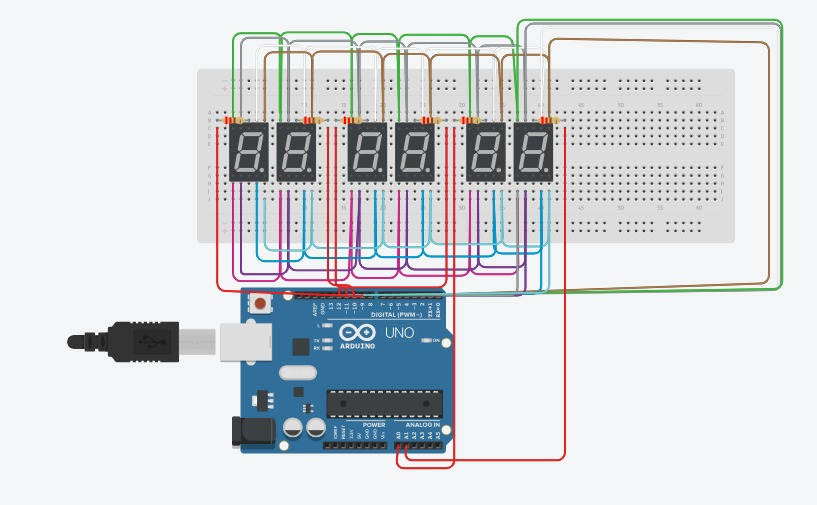
\includegraphics[width=0.8\linewidth]{figs/clockcircuit.jpeg}
 \end{figure}
 After connecting the circuit upload the following code to the arduino uno.
 Refer to the file \texttt{codes/clock.c}.
 \section*{\textbf{Implementation}}
 \begin{itemize}
     \item \textbf{Multiplexing:} Since multiple digits need to be displayed with limited pins, a multiplexing technique is used to switch between digits rapidly.
     \item \textbf{Timing Mechanism:} Implemented using AVR timers to generate 1-second intervals for updating the clock.
    \item \textbf{Digit update logic:}The digits are refreshed periodically to maintain a stable visual output without flickering.
 \end{itemize}
\section*{\textbf{Challenges and Solutions}}
\begin{itemize}
    \item \textbf{Limited Arduino pins:}Managed by optimizing connections and implementing multiplexing.
    \item \textbf{Accurate timing:}Utilized software counters and hardware timers to maintain precise 1-second intervals
\end{itemize}
\section*{\textbf{Conclusion}}
The digital clock successfully displays the current time using a 7-segment display and updates in real-time. The use of multiplexing and AVR timers ensures efficient performance. 
\end{document}
